\chapter{Ultrafast E$_{11}$ Exciton Quenching in (6,5) SWCNTs After Resonant E$_{22}$ Pumping}

\section{Overview}

This chapter presents an investigation of $E_{11}$ exciton quenching in (6,5)-enriched suspensions using optical-pump, white-light probe measurements. The samples studied include a suspension of (6,5)-enriched SWCNTs dispersed using sodium deoxycholate (DOC) in an aqeuous solution, and enriched using gel chromatography (Section \ref{sec:aqueous_susp}) and another suspension of (6,5)-enriched SWCNTs that were dispersed in toluene using the polymer PFO-BPy (Section \ref{sec:polymer_susp}). All measurements were taken with optical pump photon energy equaling that of the $E_{22}$ resonance at 2.17 eV. Moreover, the measurements were conducted at room temperature under ambient conditions.

For the DOC-suspended sample, the aqueous solution slowly evaporated over time due to a crack in the quartz cuvette containing the dispersion. As a result, the concentration of SWCNTs steadily increased over time leading to an overall increase in optical absorption. This was accounted for by measuring the sample attenuance before each experiment to normalize the experimental data to ensure the consistency of the date. In comparison, the polymer-wrapped sample was well sealed and no significant changes in the sample absorption were observed over time.


\section{Experimental Results}

\subsection{DOC-Suspended (6,5)-Enriched Suspension}

Figures \ref{fig:weilu_cnt_time_traces} $-$ \ref{fig:weilu_cnt_normalized_dt} present data obtained for the DOC-suspended sample. In particular, Figure \ref{fig:weilu_cnt_time_traces} shows the normalized attenuance of the sample at indicated time delays using a pump power density of 7.82 GW/cm$^2$. This shows that a very fast response occurred at the $E_{11}$ resonance shortly after the sample was resonantly excited at the $E_{22}$ transition. Figure \ref{fig:weilu_cnt_max_decay} shows the maximum decay of the total attenuance within the spectral region of the $E_{11}$ resonance. Here, the oscillator strength of the $E_{11}$ resonance diminishes further as the optical pump intensity increases and the peak almost completely disappears at the highest power density.

Figure \ref{fig:weilu_cnt_max_decay_fit} shows the peak attenuance obtained in Figure \ref{fig:weilu_cnt_max_decay} as a function of the power density of the optical pump. Initially, the peak attenuance decreases linearly until it begins to saturate at power densities above 7.8 GW/cm$^2$. Furthermore, Figure \ref{fig:weilu_cnt_normalized_dt} shows the normalized differential transmission curves measured at the labeled power densities. These curves were fit using a bi-exponential decay model to obtain decay constants. Figure \ref{fig:weilu_cnt_decay_const} shows the fast and slow decay constants extracted from the fits shown in Figure \ref{fig:weilu_cnt_normalized_dt}(a). The fast decay constant increases linearly, whereas the trend exhibited by the slow decays is more difficult to interpret.

\begin{figure}[H]
	\centering
	{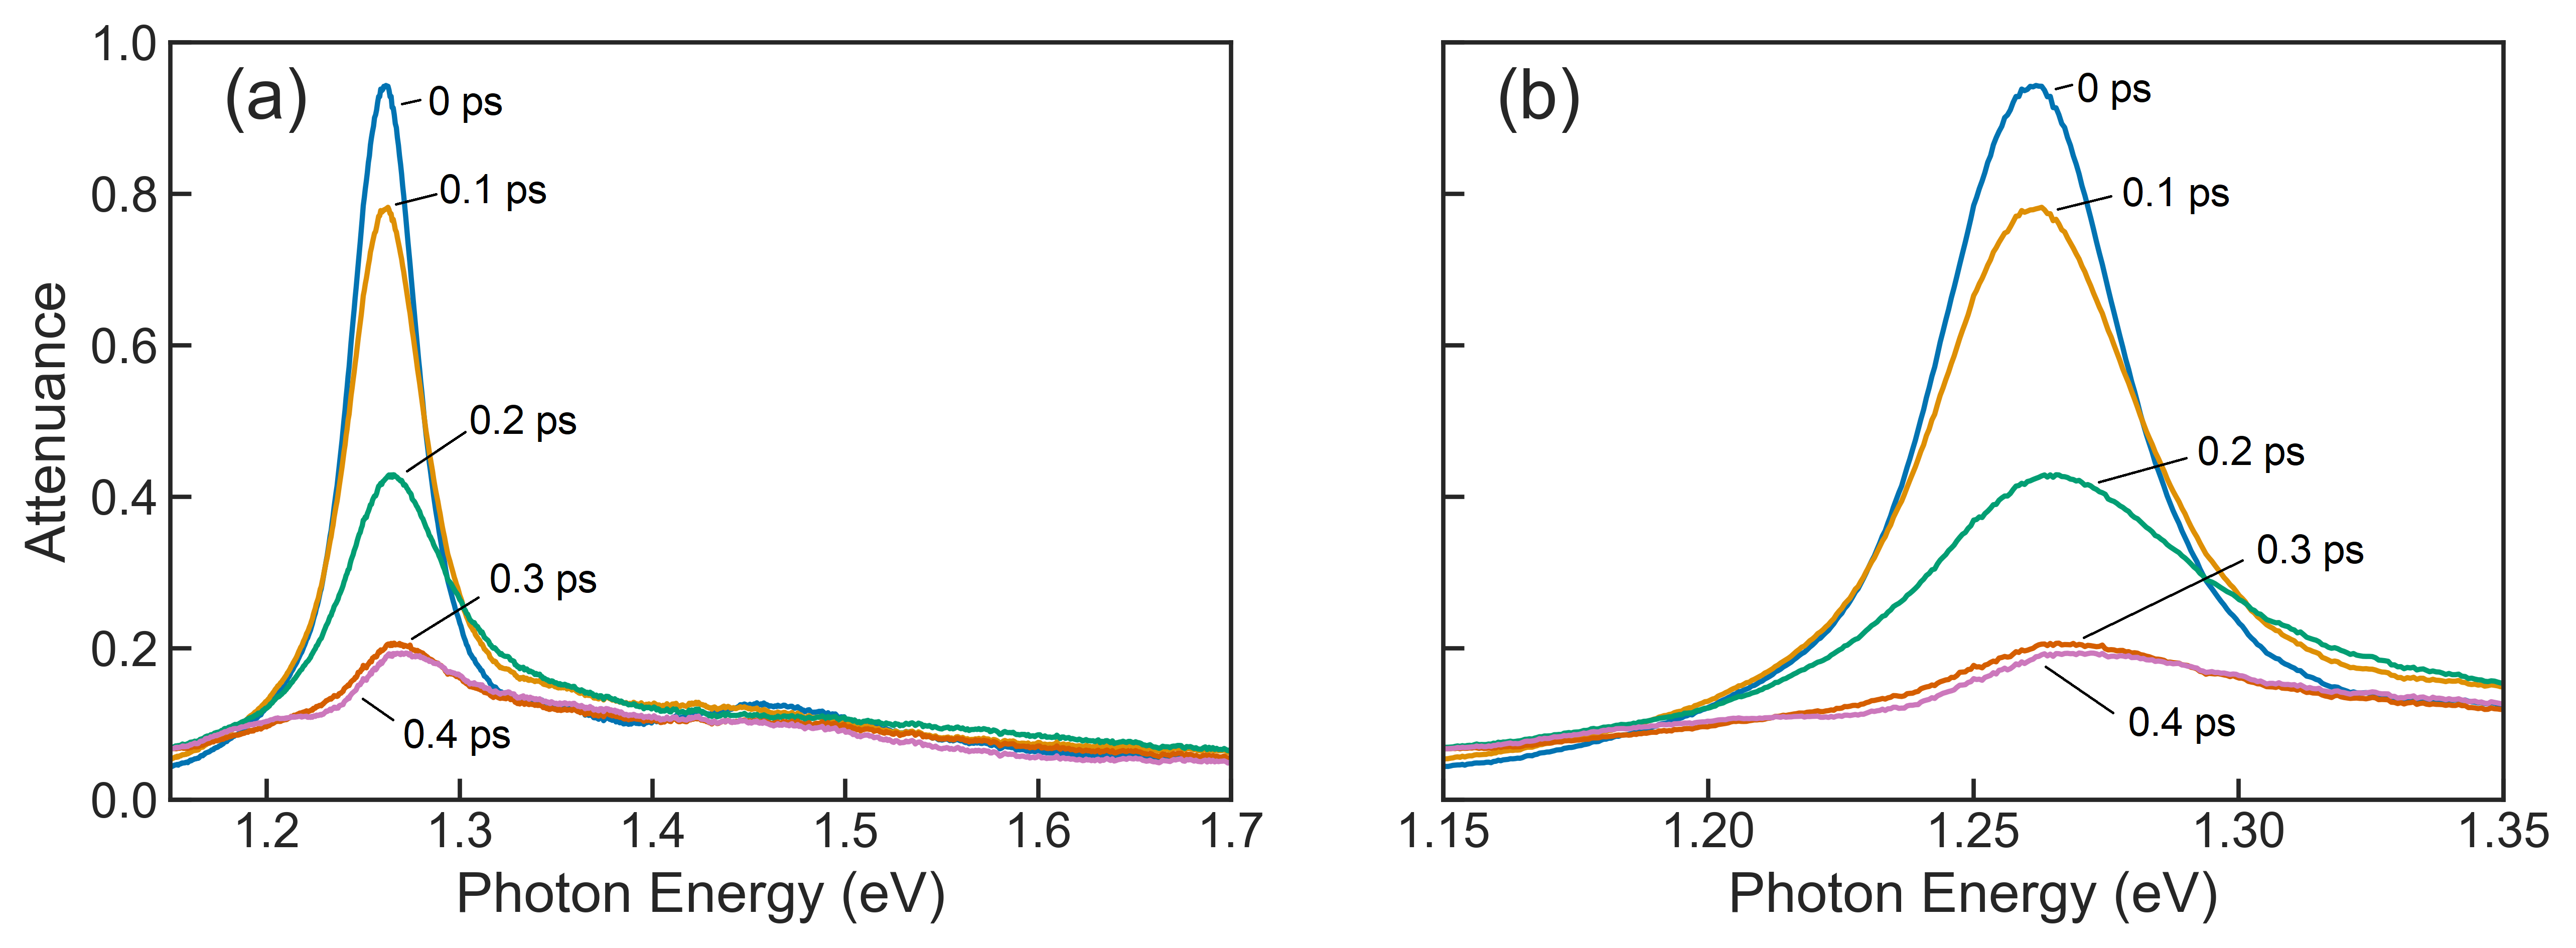
\includegraphics[height=2.4in]{images/chapter_my_data/Weilu_CNT_4mW_E11_decay_relabeled} \phantomsubcaption}
	{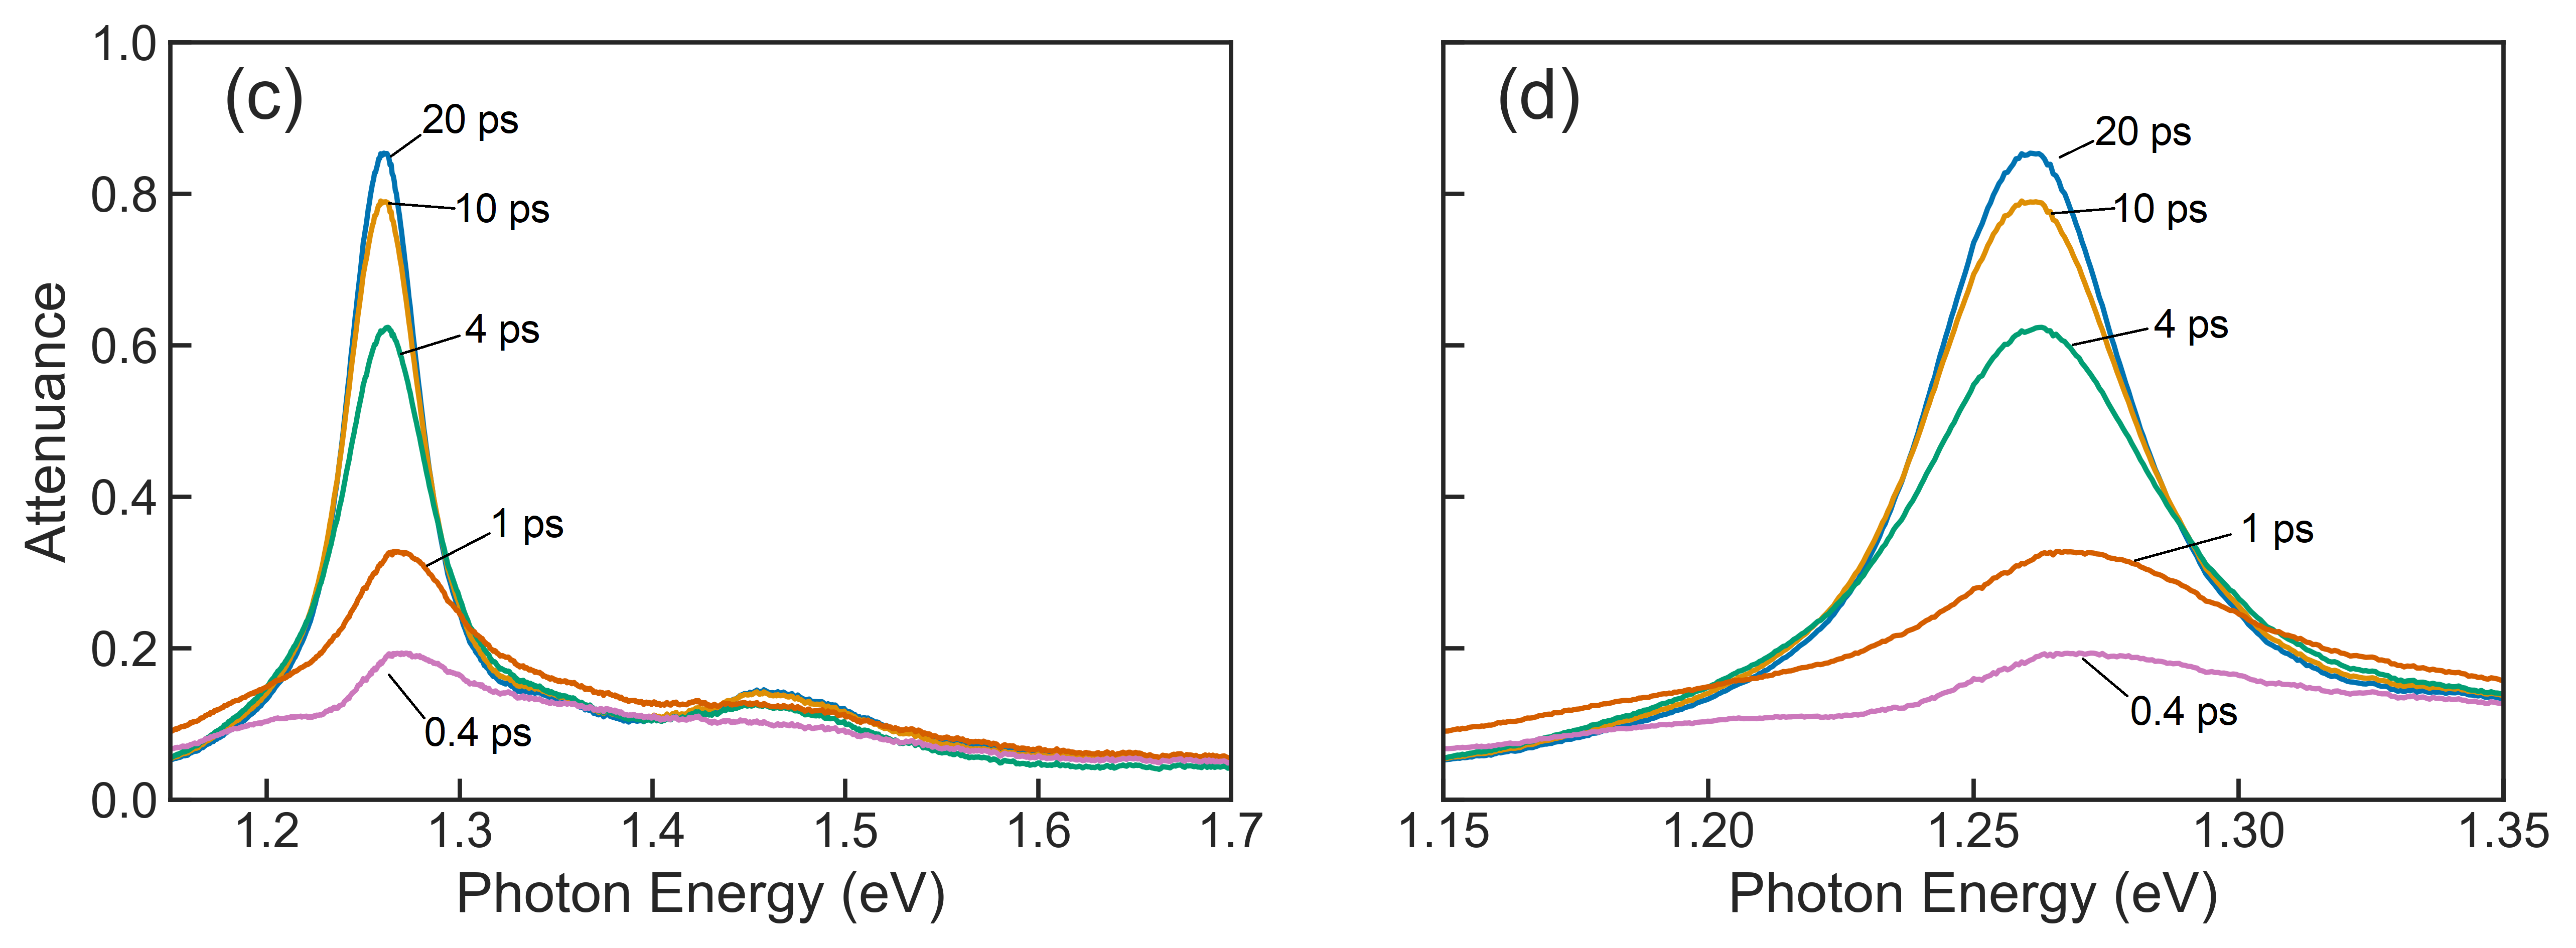
\includegraphics[height=2.4in]{images/chapter_my_data/Weilu_CNT_4mW_E11_recovery_relabeled} \phantomsubcaption}
	\caption{Normalized attenuance traces measured for the DOC-suspended SWCNTs, at the indicated time delay after resonantly exciting the $E_{22}$ transition with a power density of 7.82 GW/cm$^2$. (a) Total attenuance showing the decay of the absorption at the $E_{11}$ peak at 1.26 eV as well as the attenuation of the phonon sideband located at 1.35 eV. (b) A close-up of the changes $E_{11}$ spectral region shown in Figure (a). (c) Total attenuance at later times showing the recovery of the $E_{11}$ and phonon sideband peaks. (d) A close-up of the changes $E_{11}$ spectral region shown in Figure (c).}
	\label{fig:weilu_cnt_time_traces}
\end{figure}

\begin{figure}[ht]
	\centering
	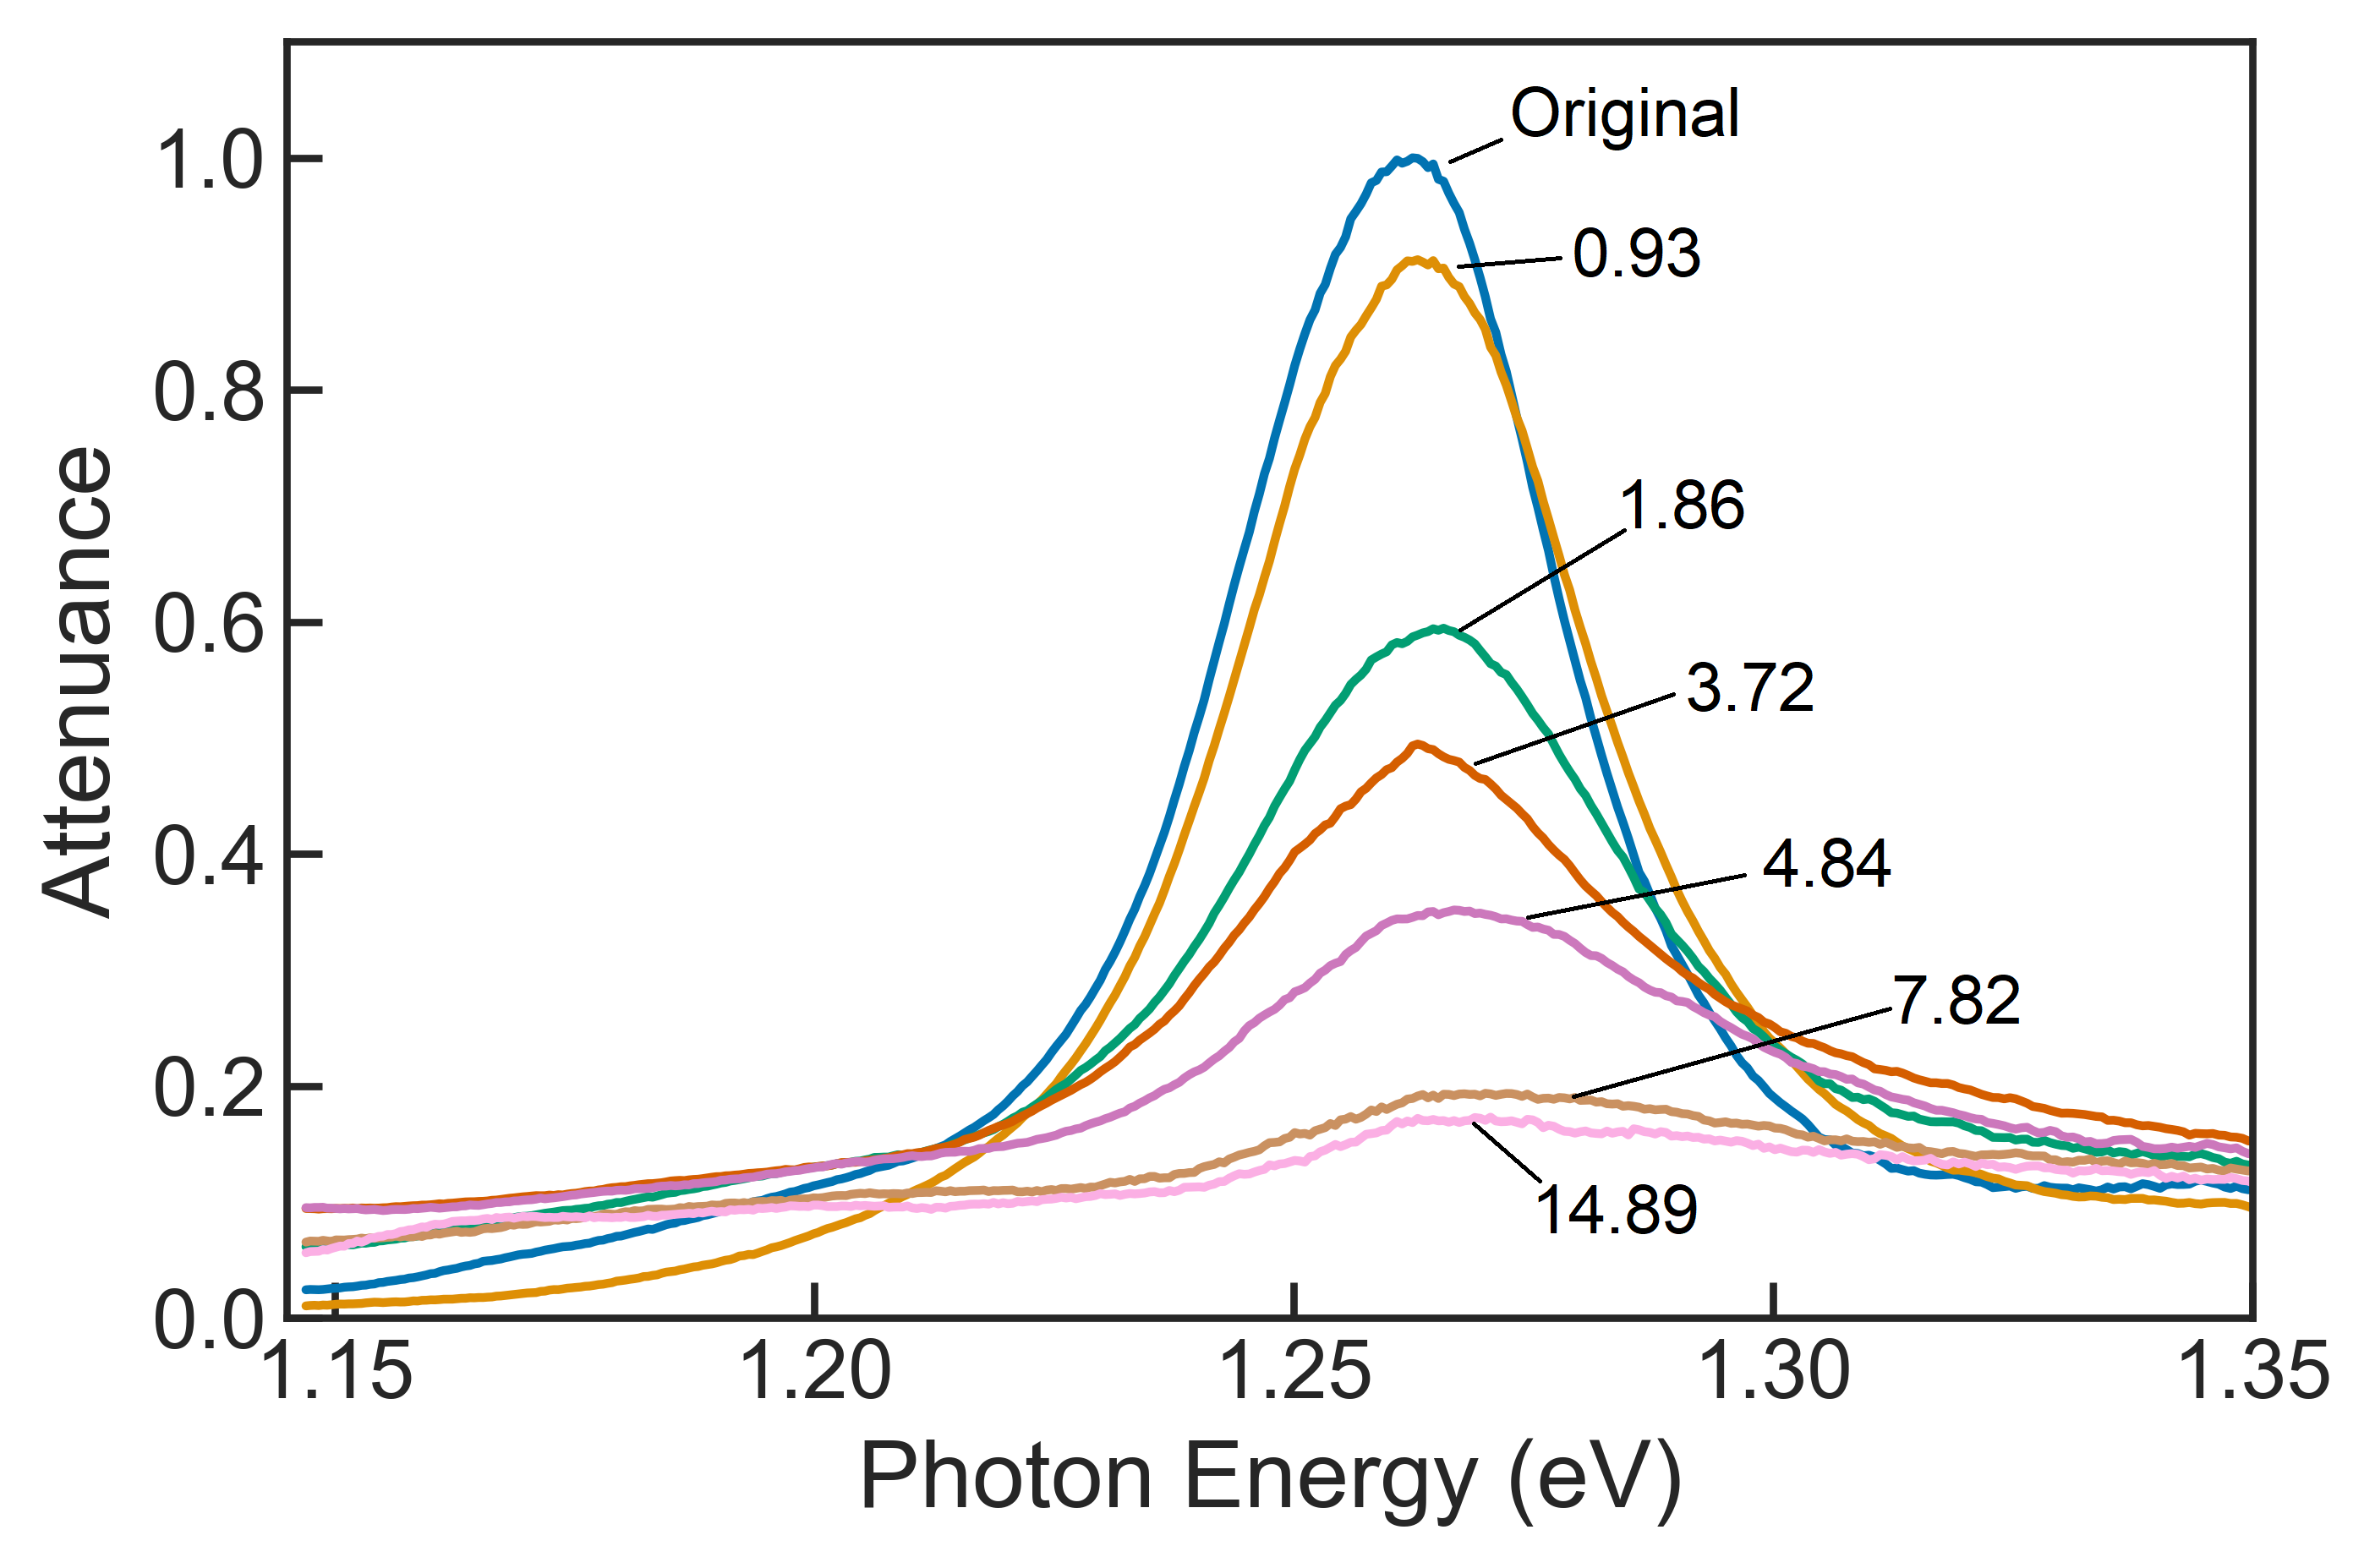
\includegraphics[height=2.4in]{images/chapter_my_data/Weilu_CNT_abs_max_change_relabeled}
	\caption{Maximum decay of the $E_{11}$ peak for the DOC-suspended SWCNTs, observed at the labeled excitation power densities (GW/cm$^2$). The top-most trace shows the linear absorption of the spectral region. At higher power densities, the $E_{11}$ resonance diminishes more and more due to the creation of carriers. The peak also slightly blueshifts and broadens.}
	\label{fig:weilu_cnt_max_decay}
\end{figure}

\begin{figure}[H]
	\centering
	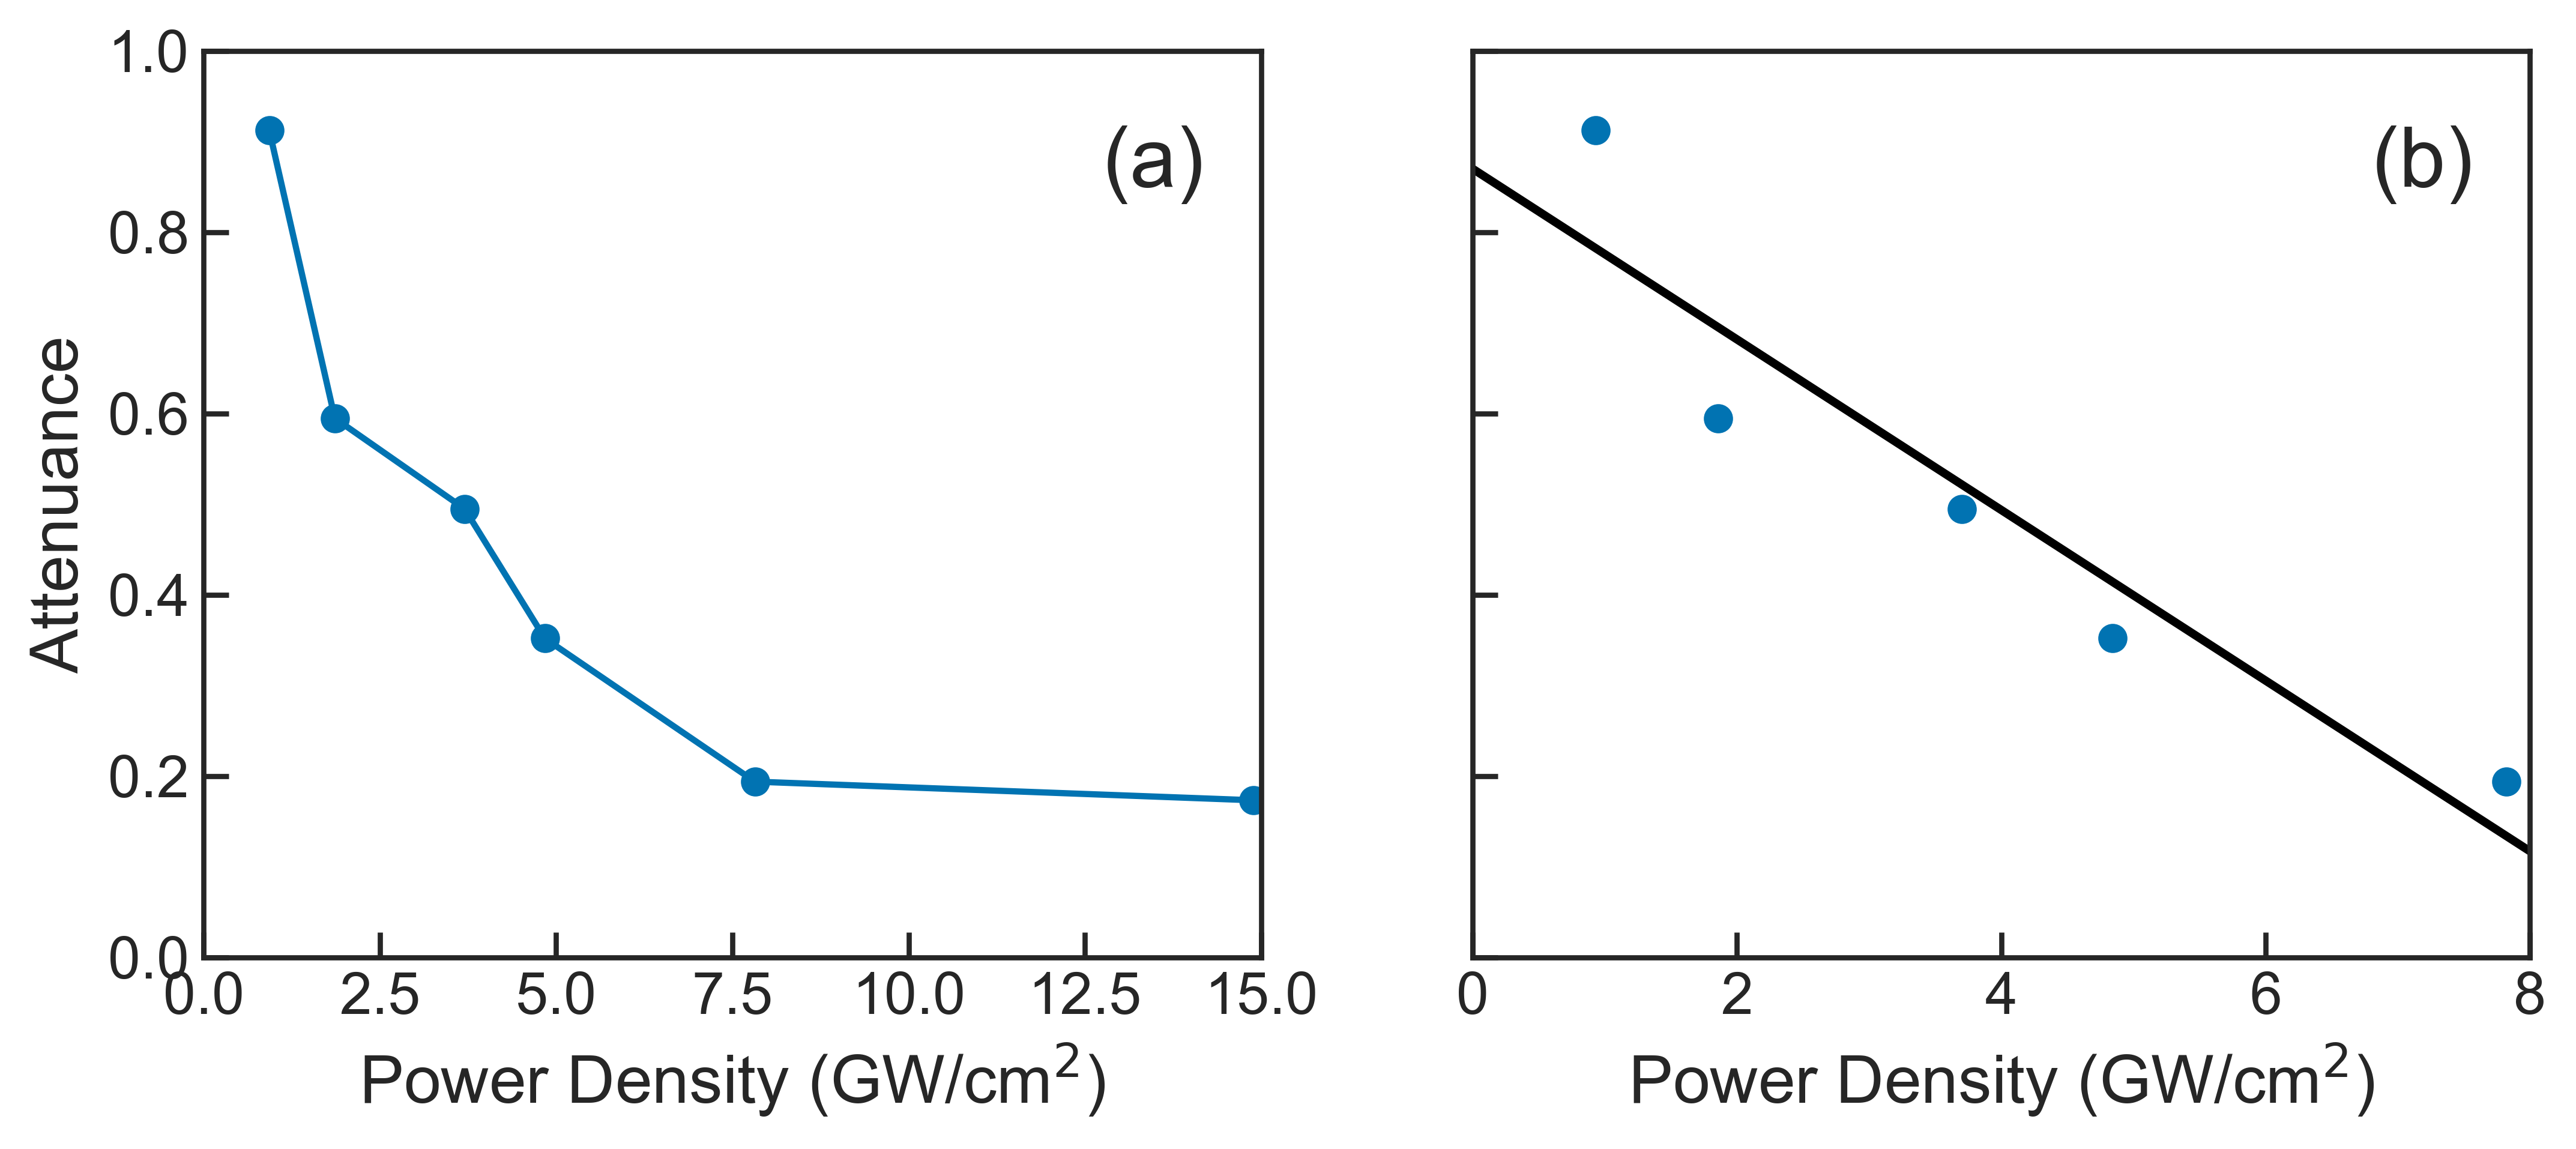
\includegraphics[height=2.4in]{images/chapter_my_data/Weilu_CNT_max_attenuance_and_fit}
	\caption{Maximum attenuance of the $E_{11}$ peak for the DOC-suspended SWCNTs, as a function of power density obtained from Figure \ref{fig:weilu_cnt_max_decay}. (a) Photo-bleaching of the $E_{11}$ resonance appears to saturate above a power density of 8 GW/cm$^2$. (b) Below power densities of 8 GW/cm$^2$, the decay of the $E_{11}$ peak is linearly proportional to the power density.}
	\label{fig:weilu_cnt_max_decay_fit}
\end{figure}

\begin{figure}[ht]
	\centering
	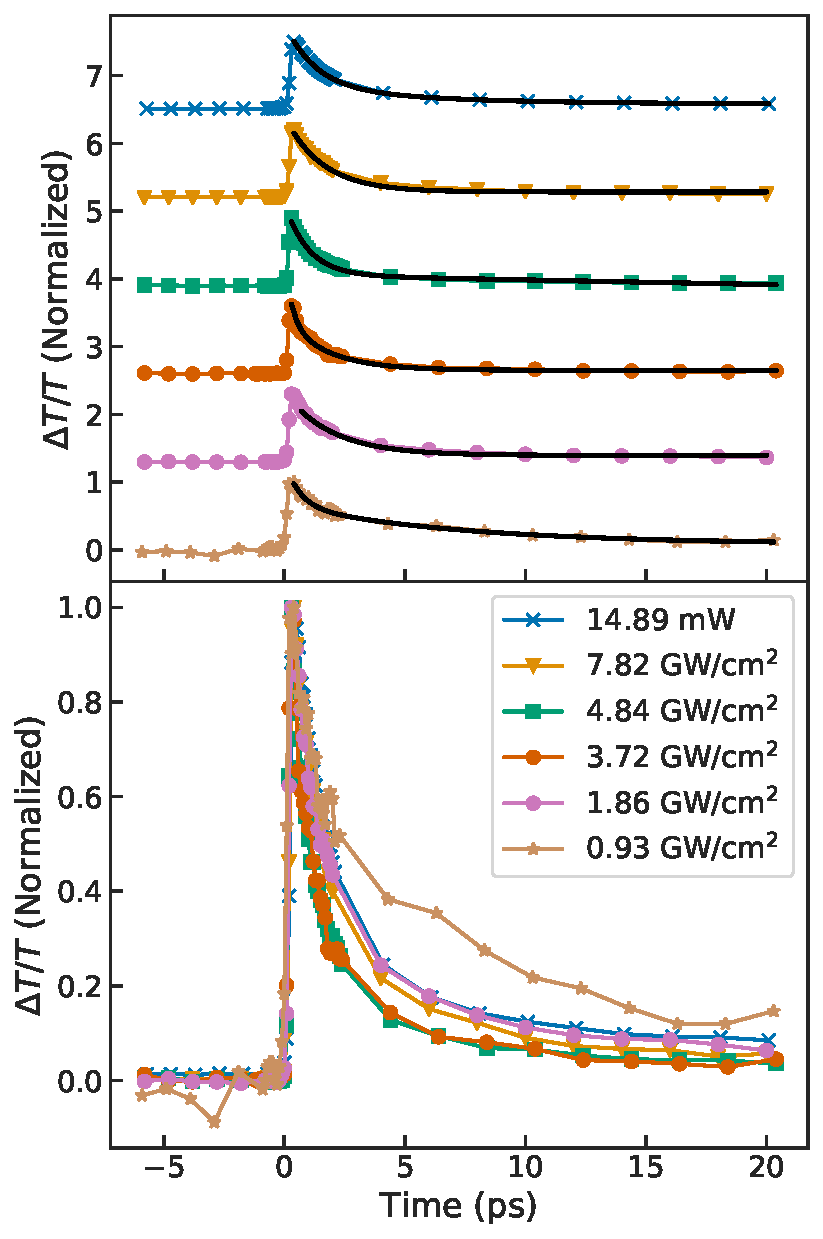
\includegraphics[height=5.4in]{images/chapter_my_data/Weilu_CNT_diff_trans_fits_and_normalized}
	\caption{ Normalized differential transmission measured at the $E_{11}$ resonance for the DOC-suspended SWCNTs, at the labeled power densities. (a) Each curve is manually offset for clarity. The solid black lines correspond to fits to the data using a bi-exponential decay model. (b) The differential transmission does not appear to have a significant dependence on the pump power density especially at higher intensities. The dynamics at the lowest intensity are dominated by the slower decay process. At higher intensities, all the measured traces do not show significant deviations from each other as expected from the effects of efficient exciton-exciton annihilation. }
	\label{fig:weilu_cnt_normalized_dt}
\end{figure}




\begin{figure}[ht]
	\centering
	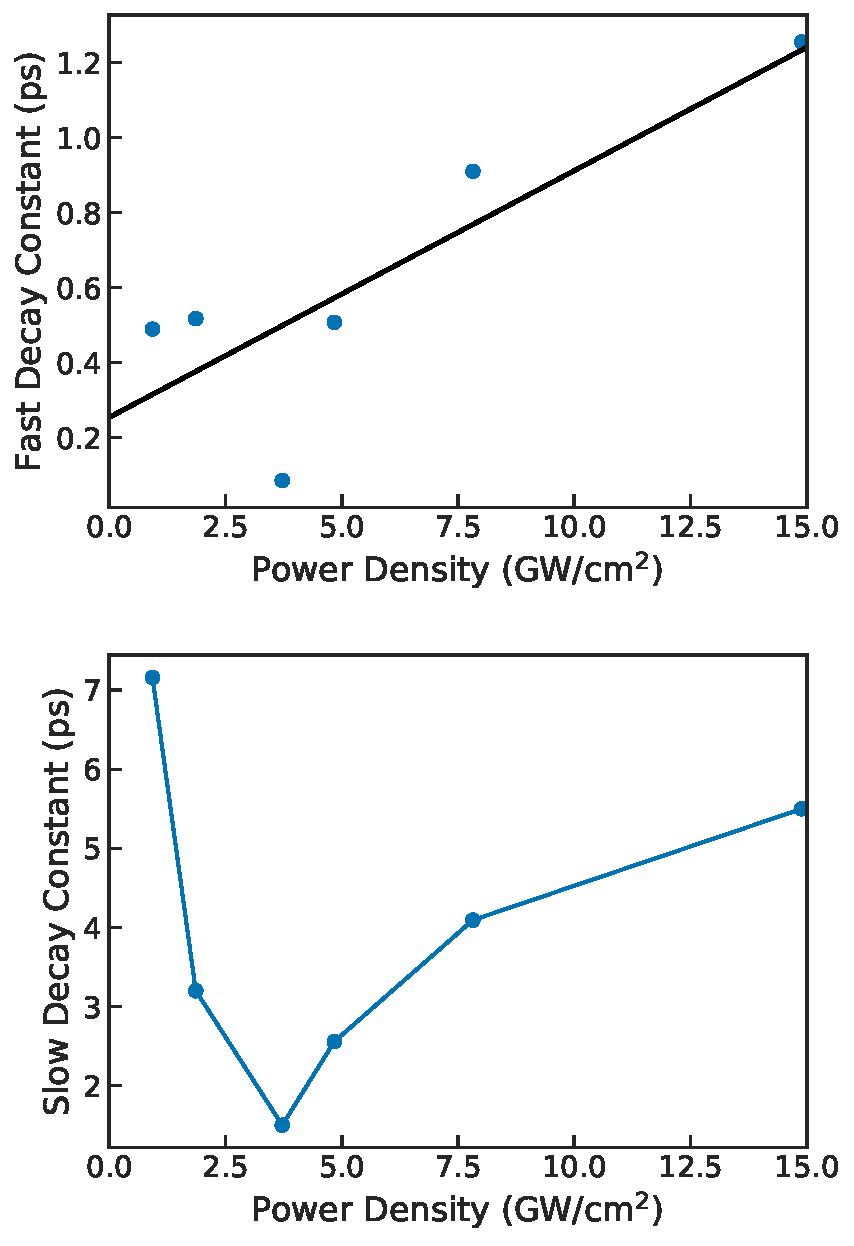
\includegraphics[height=5.4in]{images/chapter_my_data/Weilu_CNT_Fast_Slow_Decay_Const}
	\caption{(a) Fast and (b) slow decay constants extracted from the fits to the data shown in Figure \ref{fig:weilu_cnt_normalized_dt}(a). The the fast decay constant increases linearly with with the power density. This does not corroborate efficient exciton-exciton annihilation, where the fast decay constant would be expected to decrease with the power density rather than increase. The slow decay constant however shows a slightly different trend. While it appears to dominate the dynamics observed at the lower power density it decreases, it diminishes at medium intensities but increases yet again at the highest intensities.}
	\label{fig:weilu_cnt_decay_const}
\end{figure}


\clearpage
\subsection{Polymer-Wrapped (6,5)-Enriched Suspension}

Figures \ref{fig:jan_cnt_time_traces} $-$ \ref{fig:jan_cnt_decay_const} shows the data collected for the polymer-wrapped sample. Figure \ref{fig:jan_cnt_time_traces} shows the normalized attenuance of the sample at indicated time delays using a pump power density of 1.9 GW/cm$^2$. Here, the absorption associated with the $E_{11}$ resonance diminishes slightly. Figure \ref{fig:jan_cnt_max_decay} shows the maximum decay of the total attenuance within the spectral region of the $E_{11}$ resonance. As the optical pump intensity increases, the oscillator strength of the $E_{11}$ decreases.

Figure \ref{fig:jan_cnt_max_decay_fit} shows the peak attenuance obtained in Figure \ref{fig:jan_cnt_max_decay} as a function of the power density of the optical pump. Due to the limited data collected in Figure \ref{fig:jan_cnt_max_decay_fit} it is more difficult to conclude whether saturation does occur. However, the decrease in the attenuance appears to be somewhat linear as shown by the linear fit to the data. Figure \ref{fig:jan_cnt_max_normalized_dt} shows the normalized differential transmission curves measured at the labeled power densities. The curves were fit using a single exponential decay model. Figure \ref{fig:jan_cnt_decay_const} shows the decay constants extracted from the fits shown in Figure \ref{fig:jan_cnt_max_normalized_dt}(a). Here, the decay constant appears to not change significantly with higher optical pump intensities.



\begin{figure}[H]%
	\centering
	{\includegraphics[height=2.4in]{images/chapter_my_data/Jan_CNT_ABS_1mW_decay_relabeled} \phantomsubcaption}
	{\includegraphics[height=2.4in]{images/chapter_my_data/Jan_CNT_ABS_1mW_recovery_relabeled} \phantomsubcaption}
	\caption{Attenuance traces for the polymer-wrapped suspension, measured at the indicated time delay after resonantly exciting the $E_{22}$ transition with a power density of 1.9 GW/cm$^2$. (a) Total attenuance showing the decay of the absorption at the $E_{11}$ peak at 1.26 eV as well as the attenuation of the phonon sideband located at 1.35 eV. (b) A close-up of the changes $E_{11}$ spectral region shown in Figure (a). (c) Total attenuance at later times showing the recovery of the $E_{11}$ and phonon sideband peaks. (d) A close-up of the changes $E_{11}$ spectral region shown in Figure (c).}
	\label{fig:jan_cnt_time_traces}
\end{figure}

\begin{figure}[ht]
	\centering
	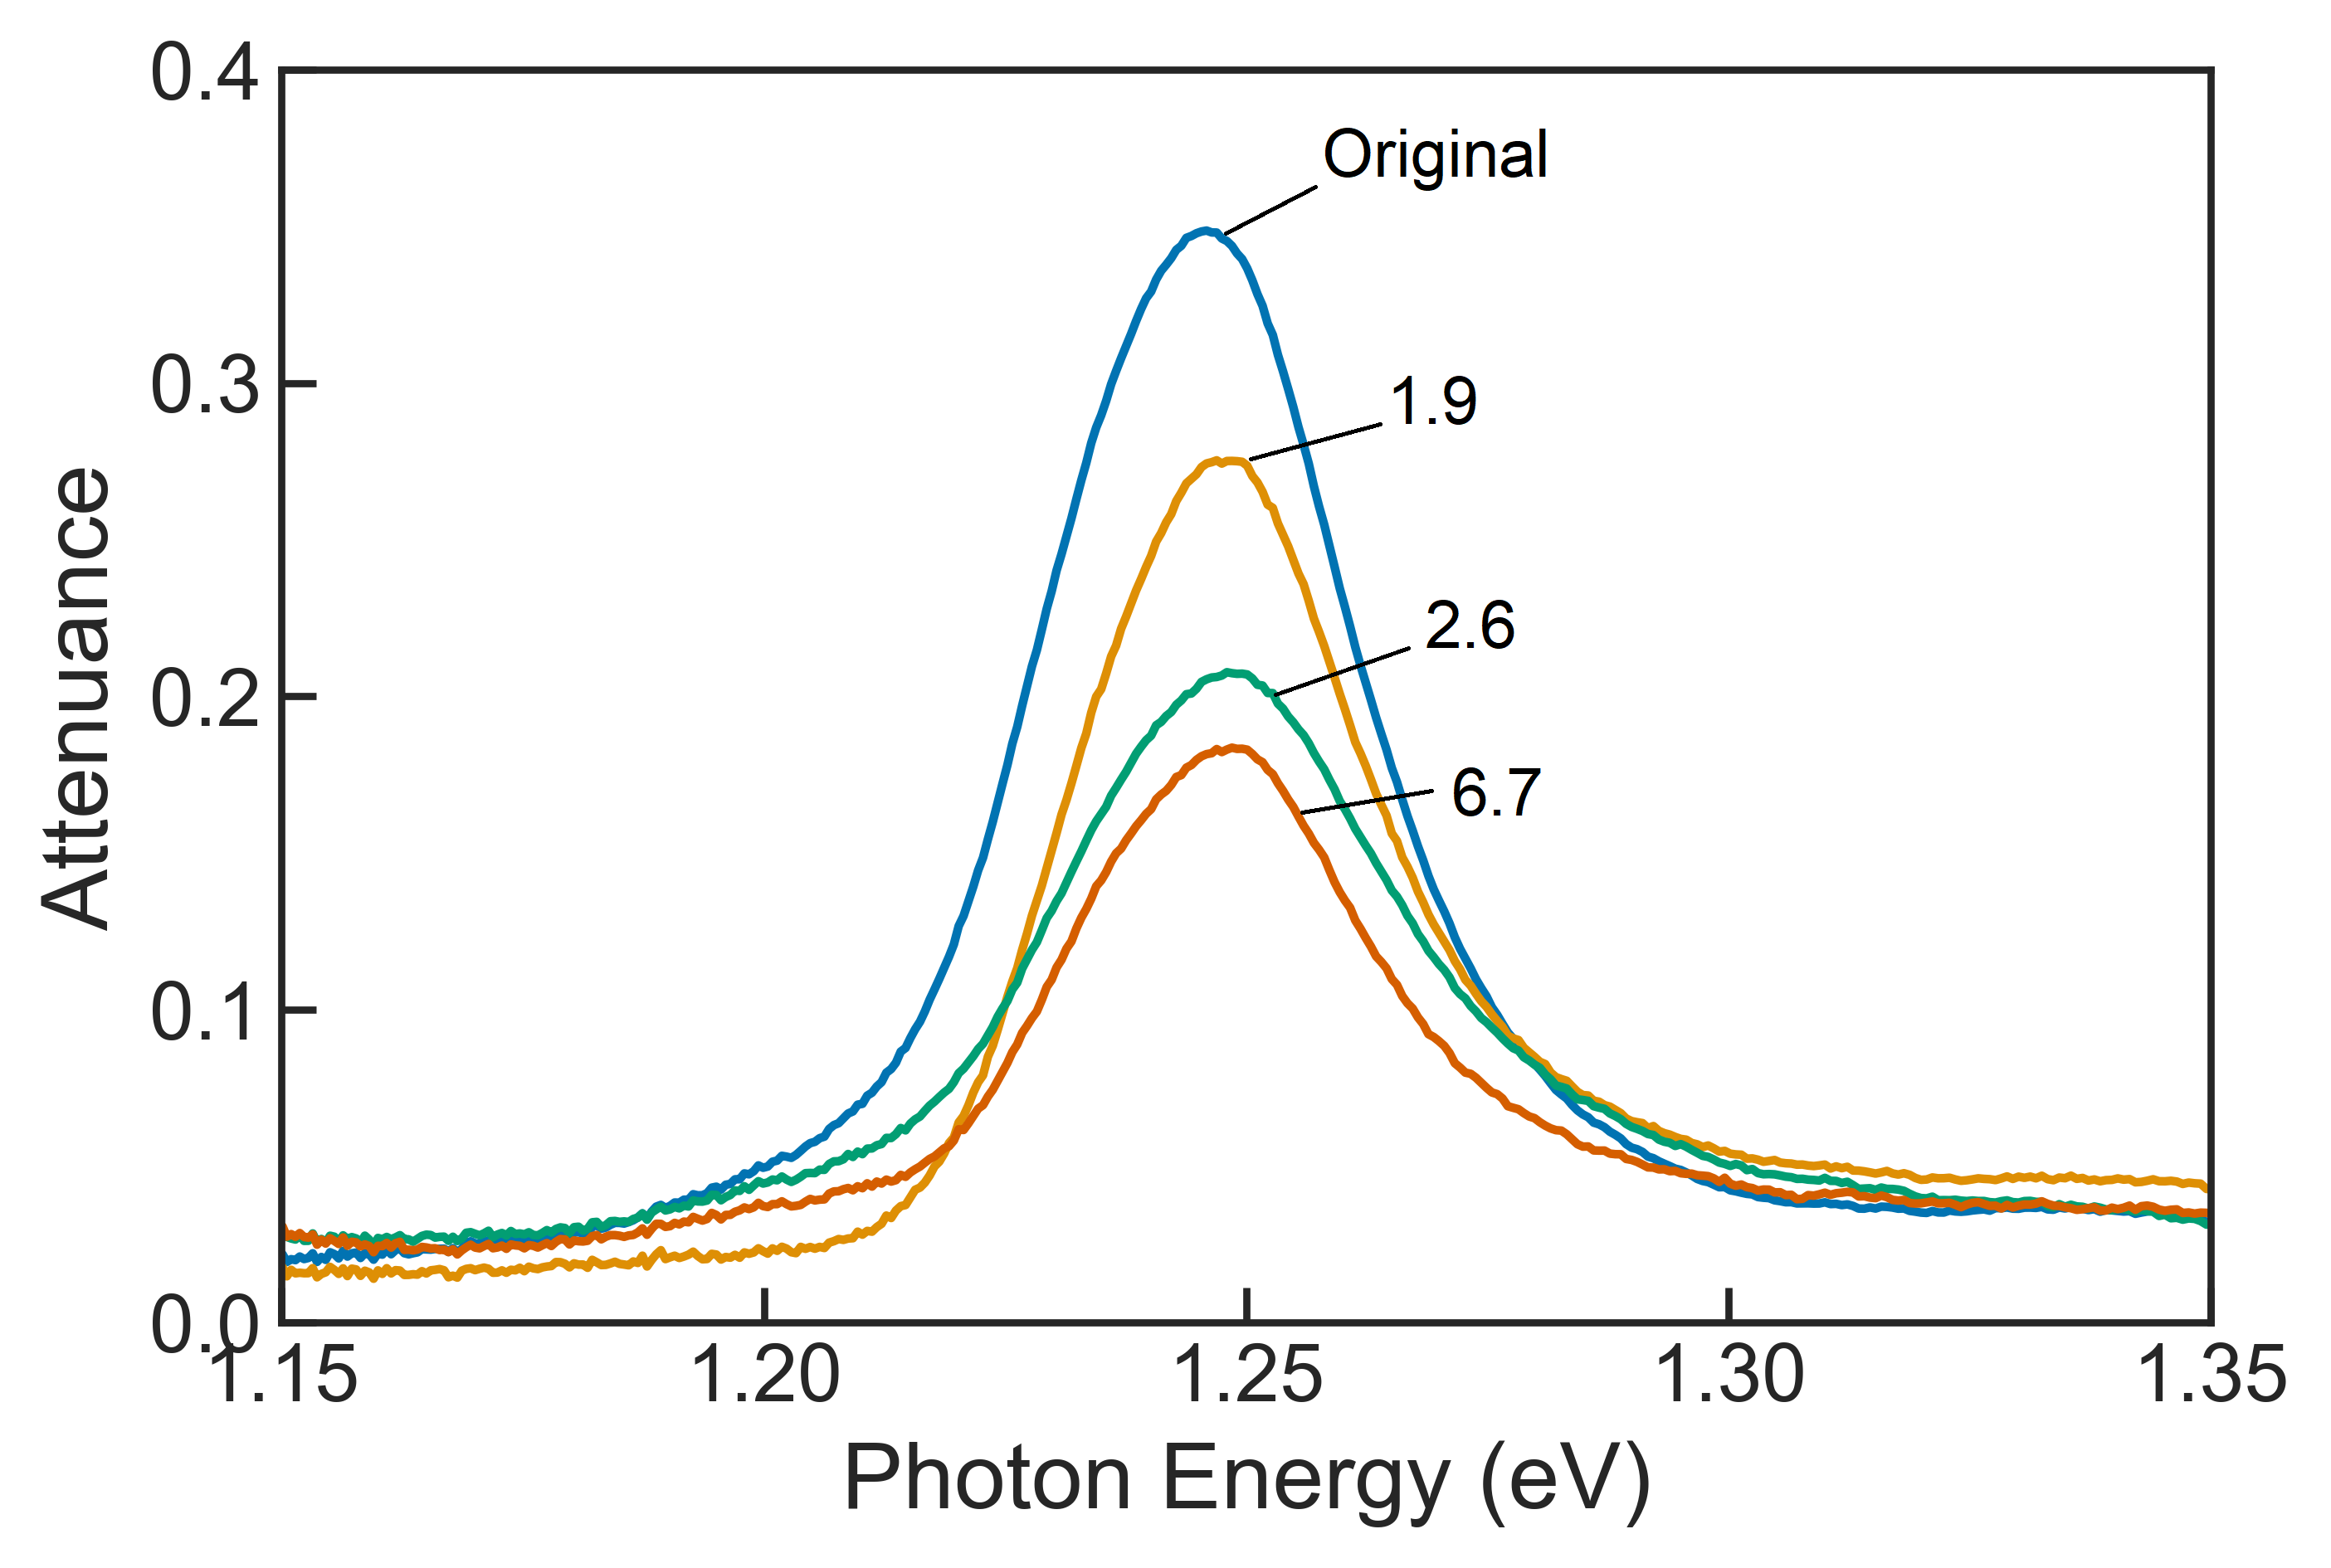
\includegraphics[height=2.4in]{images/chapter_my_data/Jan_CNT_max_abs_change_relabeled}
	\caption{Maximum decay of the $E_{11}$ peak for the polymer-wrapped sample observed at the labeled excitation power densities (GW/cm$^2$). The top-most trace shows the linear absorption of the spectral region. At higher power densities, the $E_{11}$ resonance increasingly diminishes due to the creation of carriers.}
	\label{fig:jan_cnt_max_decay}
\end{figure}

\begin{figure}[H]
	\centering
	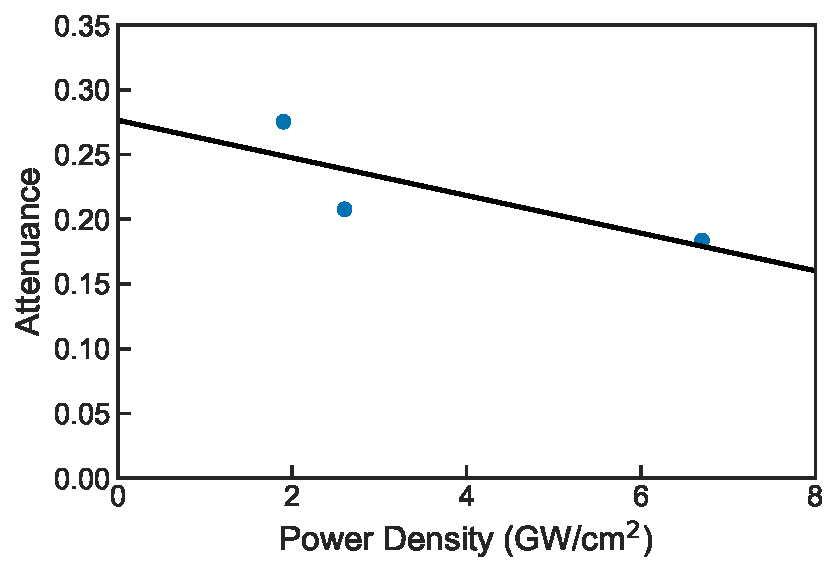
\includegraphics[height=2.4in]{images/chapter_my_data/Jan_CNT_max_attenuance_and_fit}
	\caption{Maximum attenuance of the $E_{11}$ peak for the polymer-wrapped sample, as a function of power density obtained from Figure \ref{fig:jan_cnt_max_decay}. The attenuance appears to decrease with the power density in a linear fashion.}
	\label{fig:jan_cnt_max_decay_fit}
\end{figure}

\begin{figure}[ht]
	\centering
	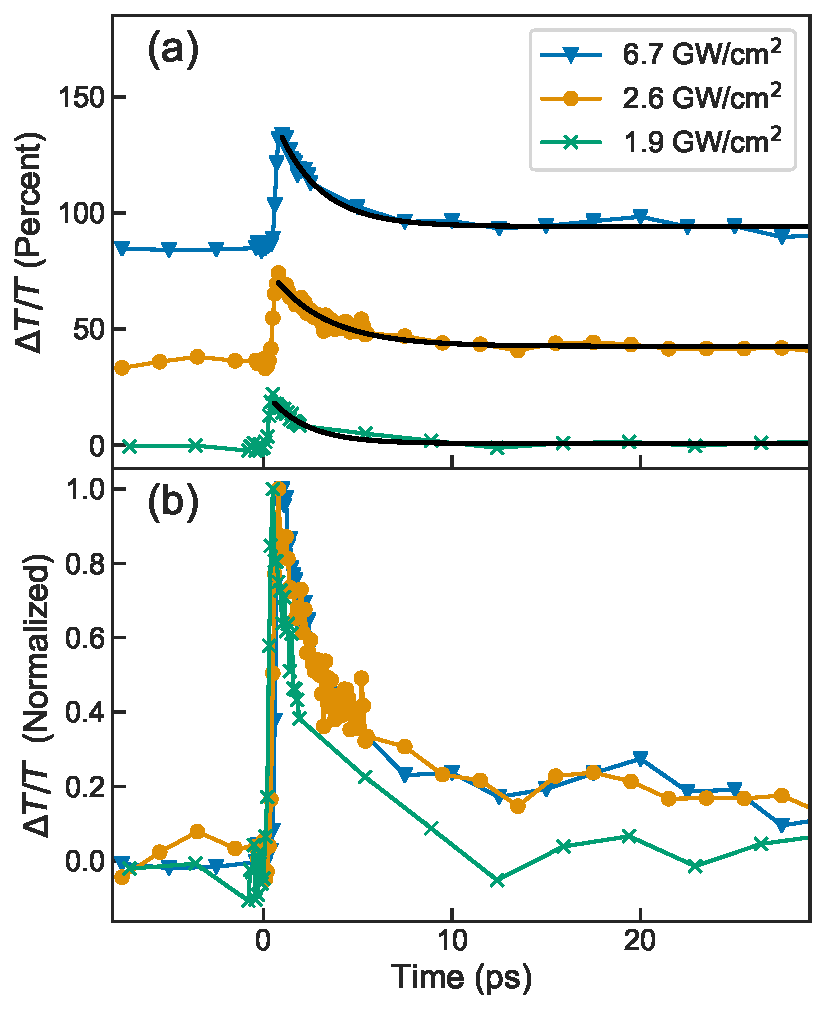
\includegraphics[height=4.4in]{images/chapter_my_data/Jan_CNT_diff_trans_fits_and_normalized}
	\caption{(a) Differential transmission measured at the $E_{11}$ resonance for the polymer-wrapped sample, at the labeled power densities. Each curve is manually offset for clarity. The solid black lines correspond to fits to the data using an exponential decay model. (b) Normalized differential transmission measured at the $E_{11}$ transition. The traces do not appear to show a significant dependence on the power density of the optical pump. Furthermore, the signals measured at 2.6 GW/cm$^2$ and 6.7 GW/cm$^2$ overlap each other.}
	\label{fig:jan_cnt_max_normalized_dt}
\end{figure}

\clearpage

\begin{figure}[ht]
	\centering
	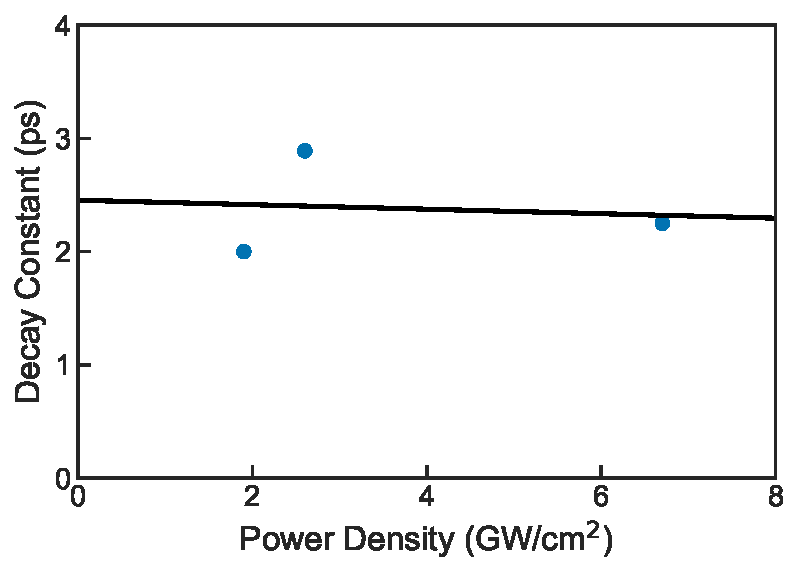
\includegraphics[height=2.5in]{images/chapter_my_data/Jan_CNT_decay_const_fit}
	\caption{Exponential decay constants obtained from Figure \ref{fig:jan_cnt_decay_const}. The decay constants do not show a significant dependence on the power density of the optical pump. }
	\label{fig:jan_cnt_decay_const}
\end{figure}

\section{Discussion }


Figures \ref{fig:weilu_cnt_time_traces} (DOC-suspended sample) and \ref{fig:jan_cnt_time_traces} (Polymer-wrapped sample) both show that $E_{22}$ excitons quickly decay to form $E_{11}$ excitons. This observation agrees with work of Manzoni \textit{et al}.\ \cite{manzoni2005intersubband} who observed that intersubband relaxation occurs on a femtosecond timescale. The two figures also do show some key differences. In Figure \ref{fig:weilu_cnt_time_traces}, the $E_{11}$ peak broadens and blueshifts. This is typically interpreted as an indication of exciton-exciton screening \cite{shah1996ultrafast}. In the presence of a large population of excitons, the Coulomb interactions between electrons and holes become screened. This leads to a reduced binding energy and broadening of $E_{11}$ peak due to the lower stability of excitons. These results differ from the observations by Ostojic \textit{et al}.\ \cite{ostojic2005stability} as well as Murakami and Kono (2009) \cite{murakami2009existence} who did not observe any change in the positions and linewidths of the optical resonances in their samples.

If exciton-exciton annihilation were indeed efficient, then the significant photo-bleaching of the optical resonances in SWCNTs should not at all be possible as mentioned by Murakami and Kono (2009) \cite{murakami2009existence}. Furthermore, the strong attenuation of oscillator strength of the $E_{11}$ peak for the DOC-suspended SWCNTs may suggest that the density of photo-generated excitons exceeds the Mott density of the system. Excitons, being composed of two half-integer spin quasiparticles, are expected to behave as bosons \cite{Ashcroft, laikhtman2007excitons}. Hence, there should not be photo-bleaching of resonance if only excitons are created by the optical pump as bosons are exempt from the Pauli exclusion principle. The results here suggest that Fermions also play a role in the observed carrier dynamics. In contrast, the data for the polymer-wrapped sample shown in Figure \ref{fig:jan_cnt_time_traces} instead shows a narrowing of the $E_{11}$ resonance, especially on the lower energy region of the $E_{11}$ resonance. This type of behavior is often interpreted as a signature of spectral hole burning but it could otherwise indicate a sign of some sort of inhomogeneity in the suspension.

Morever, the changes in differential transmission recorded at the $E_{11}$ resonance do not corroborate the previously reported evidence of efficient exciton-exciton annihilation. Figures \ref{fig:weilu_cnt_normalized_dt} (DOC-Suspended Sample) and \ref{fig:jan_cnt_max_normalized_dt} (Polymer-Wrapped Sample) demonstrate this. In Figure \ref{fig:weilu_cnt_normalized_dt}(a), DOC suspension sample showed carrier dynamics that agreed with a bi-exponential fit, whereas those of polymer-wrapped sample shown in Figure \ref{fig:jan_cnt_max_normalized_dt} instead corresponded to exponential decays. This suggests that carrier relaxation in the polymer-wrapped sample occurs more slowly at longer time delays. Overall, the normalized differential transmission data measured at the indicated power densities closely overlap one another and a fast initial decay does not dominate the observed dynamics at higher power densities. These result however may not be too surprising as previous transient absorption measurements in the literature also did not observe any nonlinear carrier dynamics associated with efficient exciton-exciton annihilation \cite{ostojic2004interband, manzoni2005intersubband, ma2005femtosecond, luer2009size}.

Furthermore, the scenario presented by dominant exciton-exciton annihilation processes suggests that the initial decay should become faster with increasing power density. The decay constants extracted from the differential transmission data do not exhibit such a trend. Figures \ref{fig:weilu_cnt_decay_const} and \ref{fig:jan_cnt_decay_const} show the extracted decay constants obtained by fitting to the differential transmission measured in each sample respectively. In Figure \ref{fig:weilu_cnt_decay_const}(a), the fast decay constant increases linearly with the power density, whereas in Figure \ref{fig:jan_cnt_decay_const} the decay time does not change significantly. One issue with Figure \ref{fig:jan_cnt_decay_const} however, is that more data points would be needed at lower and higher optical pump intensities to give more confidence to this claim. It may already be the case that the optical pump was strong enough to directly put the system in a regime of efficient exciton-exciton annihilation.

With regards to whether an exciton Mott transition can be achived in SWCNTs, the data shown here raise an important question. Namely, why is it that $E_{11}$ exciton quenching was easily achieved in the DOC-suspended SWCNTs, whereas the polymer-wrapped SWCNTs did not exhibit such behavior? Indeed, these results mirror some of the experimental observations reported by Ohno \textit{et al.} \cite{ohno2007excitonic}, as discussed in Section \ref{sec:diff_exc_annih}. In brief, they conducted time-resolved photoluminescence experiments where they observed a bi-exponential decay for SWCNTs that were immersed in air. However, a single exponential decay was observed for SWCNTs that were instead immersed in hexane. The difference in the dielectric environments of the SWCNTs clearly played a role in carrier dynamics that were observed as the dielectric constant of hexane ($\epsilon$ = 1.9) is higher than that of air ($\epsilon = 1$).

A similar observation can be made regarding the samples used in this study. From the optical absorption spectrum, shown in Figure \ref{fig:abs_comp_normalized}, it is clear that the SWCNTs of the polymer-wrapped sample are immersed in an environment with a higher dielectric constant. The resonances of the polymer-wrapped sample are redshifted relative to those of the DOC-suspended SWCNTs (Section \ref{section:dielectric_screening}). Indeed, it is already known that the dielectric constant of toluene is 2.25, whereas the dielectric constant of water is 1.76 \cite{samoc2003dispersion}. Furthermore, the fact that the polymer-wrapped sample exhibits a faster intial decay could be a sign of efficient exciton-exciton annihilation given that the attenuance spectrum appears to be saturating. Yet, this decay time does not show a clear trend of decreasing as the optical pump intensity increases, as shown in Figure \ref{fig:jan_cnt_decay_const}. This may however corroborate the hypothesis posed by Ohno \textit{et al}.\ who suggested that non-radiative decay centers may be created at the interface of the SWCNTs and their surrounding medium.

In reconciling the results presented here with the current literature, there are two particular parameters that need to be accounted for. According to diffusion-limited exciton-exciton annihilation, two relevant length scales include SWCNT lengths and exciton correlation lengths (Section \ref{sec:diff_exc_annih}). Current literature has shown that SWCNT lengths can vary significantly depending on how the SWCNTs are processed as shown by Graf \textit{et al}. \cite{graf2016large} (Section \ref{sec:polymer_susp}). In addition, exciton correlation lengths can vary from sample to sample. For instance, Mann \textit{et al}.\ \cite{mann201613} measured an exciton size of  13 nm exciton size in their (6,5)-enriched suspension, using the same technique described by Luer \textit{et al}.\ \cite{luer2009size} who instead obtained an exciton size of 2 nm in their (6,5)-enriched suspension. This detail is notable as the size of excitons is expected to scale with the external dielectric constant in an approximately linear fashion \cite{perebeinos2004scaling}.   %Furthermore, Ostojic \textit{et al}.\ used a technique where calculated density of excitons created by optical pump in semiconducting SWCNTs. Sample contained metallic SWCNTs, which could absorb photons via two-photon absorption, suggesting that their own estimate of 2 nm exciton size may be a underestimate.

\begin{figure}[H]
	\centering
	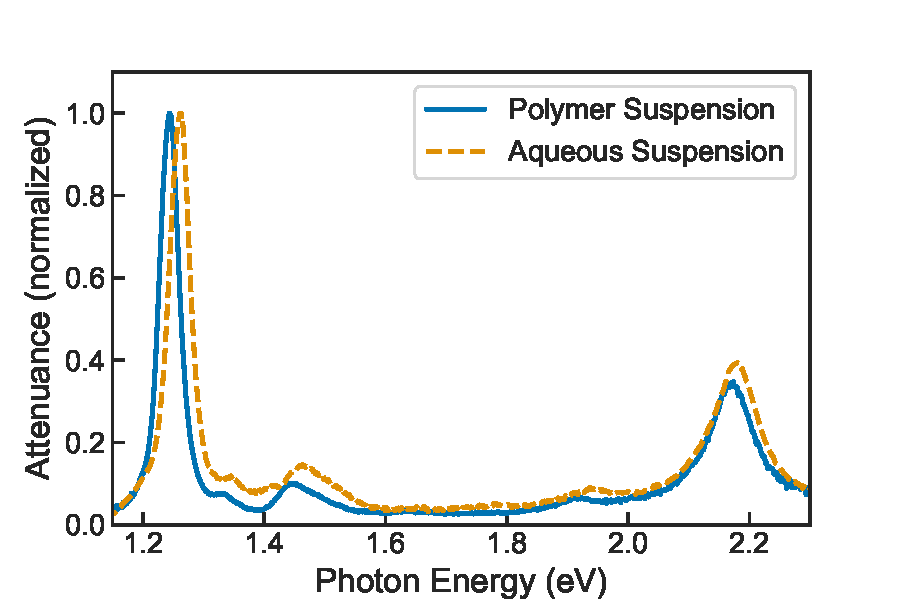
\includegraphics[scale=0.8]{images/chapter_my_data/abs_normalized}
	\caption{Normalized attenuance spectrum for the DOC-suspended sample and the polymer-wrapped sample. The spectrum for the polymer suspension is redshifted relatived to that of the aqueous suspension due to the difference in the dielectric environments of these samples. This suggests that excitons for SWCNTs in the polymer suspension are more screened by the dielectric environment (Section \ref{section:dielectric_screening}).}
	\label{fig:abs_comp_normalized}
\end{figure}


At a first glance, it is intuitive to think that if the exciton binding energy is reduced by the screening of the dielectric environment, then the Mott density should also decrease. However, one hypothesis for why it would be harder to achieve an exciton Mott transition is that if excitons are larger, then the system may be more prone to exciton-exciton annihilation. In this regime, excitons would only need to diffuse over much shorter distances before encountering a neighboring exciton. This suggests that for SWCNTs immersed in envrionments with higher external dielectric constants, it would be harder to create a density of excitons capable surpassing the Mott density. Correspondingly, SWCNTs in environments with lower dielectric constants will exhibit smaller excitons for which exciton-exciton annihilation processes would be more so limited by diffusion processes. For such SWCNTs, it would then be easier to create a large density of excitons.

However, one issue with theoretical studies regarding the dielectric envrionment's effect on SWCNT properties is that they assume that the external dielectric constant does not vary in space \cite{perebeinos2004scaling, walsh2007screening, ando2011effects} (Section \ref{section:dielectric_screening}). As Deslippe \textit{et al}.\ suggest, it is not so clear whether this approximation is always suitable for studying individually-suspended SWCNTs \cite{deslippe2009electron}. For surfactant-based suspensions, the SWCNTs are suspended in water but also have micelle structures on their surfaces (Section \ref{sec:aqueous_susp}). In the case of polymer-based suspensions, polymer structures form at a fixed distance around the suspended SWCNTs (Section \ref{sec:polymer_susp}). Hence, the assumption that that the external dielectric constant does not vary in space may neglect important dielectric contributions of the molecules involved in solubizing the SWCNTs.

\section{Conclusions}

In this chapter, we studied the carrier relaxation dynamics of two ensembles of SWCNTs induced by resonant $E_{22}$ excitation. These two ensembles included SWCNTs suspended in an aqueous solution using DOC as a surfactant as well as another suspension of polymer-wrapped SWCNTs in a toluene solution. For both samples, we observed a fast response at the $E_{11}$ transition after creating $E_{22}$ excitons with the optical pump. In the DOC suspension, the $E_{11}$ peak broadened, blueshifted and was almost completely photobleached, suggesting that enough carriers were created to exceed the Mott density. However, in the polymer-wrapped sample, $E_{11}$ exciton quenching was not achieved.

In addition, the data do not show signs of efficient exciton-exciton annihilation. For the samples studied, the measurements indicate that the dominance of a fast exponential is rather weak and does not appropriately scale with the fluence of the optical pump as expected by time-resolved photoluminenscence measurements. Instead of an intial decay that becomes faster with higher pump intensities, a signature of exciton-exciton annihilation, we observed an intial decay that either slows down with increasing pump intensity or remains roughly constant depending on the sample being studied.

 Finally, the fact that $E_{11}$ exciton quenching was achieved in the DOC-suspended SWCNTs and not the polymer-wrapped SWCNTs suggests that the dielectric environment may play a role in determining the upper limit of excitons that can be created in SWCNTs. While there are some studies that explore how dielectric environments affect the otpical resonances of SWCNTs, not much work has been conducted on how they also affect carrier dynamics. On this topic, we have hypothesized that SWCNTs immersed in environments with higher dielectric constants may exhibit excitons with larger sizes that may be more prone to exciton-exciton annihilation, despite the Mott density being lower in such systems. However, this warrants further study of how different dielectric environments affect ultrafast exciton quenching in SWCNTs.
